\documentclass[a4paper,12pt]{article}

% Packages
\usepackage{graphicx}
\usepackage{amsmath}
\usepackage{geometry}
\usepackage{fancyhdr}
\usepackage{setspace}
\usepackage{float}
\usepackage{titlesec} 
\geometry{margin=1in}
\setstretch{1.5}

% Header and Footer
\pagestyle{fancy}
\fancyhf{}
\fancyhead[L]{Project 2.1 - Machine Learning Solutions for Agent Training in Unity}
\fancyhead[R]{\thepage}

% Title Formatting
\titleformat{\section}{\normalfont\Large\bfseries}{\thesection}{1em}{}

% Cover Page
\title{
    \vspace{2cm} % Adjust vertical space
    
\includegraphics[width=0.55\textwidth]{um-fse-logo.png} \\ % Add your logo here (change "logo.png" to the actual filename)
    \vspace{1cm} % Adjust vertical space after the logo
    \textbf{\Huge Project 2.1 - AI and Machine Learning
Controlling Agents in the Unity Game Engine and Applications in Video Game Development} \\
    \vspace{1cm} % Adjust vertical space
    \large 21/1/2025
}
\author{Žilinskas G., Mäntele KJJ, Goetsch E., Elkaffas SSMHO, Cioc A., \\Christoforou A., Bertini S.}
\date{}

\setlength{\parindent}{20pt}

\begin{document}

% Title Page
\maketitle
\thispagestyle{empty}
\newpage

% Table of Contents
% Start page numbering from the Table of Contents
\thispagestyle{empty}
\tableofcontents
\newpage

\setcounter{page}{1}
% 1. Introduction
\section{Abstract}
This project analyzes the feasibility of machine learning solutions for agent training in a real-time three-dimensional environment. We investigate the application and performance of Reinforcement Learning algorithms in agent training within Unity's ML-Agents framework. The approach included creating custom sensors, setting the training parameters, training the agents, and evaluating their performance using statistical techniques. We also performed experiments to find out if our generative AI could rival the performance of the traditional decision tree-based AI used in video games. Our study documents how to use Unity's ML-Agents library to train an agent, and our experiment results indicate that while generative AI is able to play our video game well from a technical perspective, it is unable to do so in a way that seems natural and immersive to the player.

\section{Introduction}
As machine learning becomes an increasingly popular field in computer science, many have started researching applications of machine learning solutions to agent training and game development. A popular game engine that offers native support for AI implementations is Unity, which allows for the development of 3D real-time video games. To train and create our agents, we made use of the Unity Machine Learning Agents Toolkit, also known as ML-Agents \cite{juliani2020unity}. This adds a collection of Deep Reinforcement Learning algorithms and environments that can be used to test them. For the purposes of our experiments, we decided to create our own custom environment for training agents and testing their behavior.

This research has numerous important implications for the field of game development.  Unity is a very popular game engine used by numerous developers, and so it is useful to know how to use its machine learning library to train an agent that can function as a non-playable character (NPC) in a video game. This would save game developers time and money, since AI trained with machine learning (what we call "generative AI") can learn to play a game on its own. This is in contrast to the "AI" traditionally used in games (what we call "normal AI"), which is a deterministic rule-based system that has to be manually designed and implemented. Developers who use generative AI would no longer have to spend time and money in manually testing and designing a normal AI system. These considerations lead us to two main research questions:

\begin{enumerate}
    \item How can machine learning solutions be used to train an agent in Unity?
    \item Can generative AI rival the performance of normal AI in a video game setting? 
\end{enumerate}

Our approach mainly consists of using ML-Agents' Reinforced Learning algorithms. Reinforced Learning works by setting up a reward structure for the machine learning model, where the model is rewarded for certain actions that bring it closer to a certain goal, and punished for certain actions that prevent it from achieving said goal. The model then uses this reward structure to optimize itself over multiple training iterations, altering its behavior such that it maximizes how much it is rewarded and how little it is punished. Instead of using one of ML-Agents' pre-made agents, we created our own prototype first person shooter (FPS) game and designed agents that can function as non-playable characters (NPCs) in our game. The machine learning model we trained on these agents could theoretically be used as (NPCs) in a fully fleshed out FPS game. How these NPCs could be implemented in such a game represents another possible avenue of research that follows from our project.

In section 3 of the report, we will describe our approach to training agents in Unity, including technical details of our implementation. These will be provided in sufficient detail to allow the reader to replicate our project. In section 4, we describe the set-up of our experiments and what we wanted to test with our experiments. In section 5, we display the results of our experiments in graph form. In section 6, we discuss the significance and limitations of our findings. 

% 2. Methods
\section{Methods}
ML-Agents trains agents by taking in input data using sensors, using that data with a machine learning algorithm to train the agent, and then having the agent perform a specific action based on the algorithm's output. By using custom sensors and specifying the actions we want the agent to take, we can specify agent behavior and training based on the task at hand.

For our custom environments, we created a rudimentary first-person shooter (FPS) game, complete with guns, bullets, health and ammo stats, and the necessary animations. In each training environment, there are two agents with guns, who both have the objective of killing the other agent. Environments also include 10 pickup spawn locations dotted across every environment, divided between 5 health pickup locations and 5 ammo pickup locations. At any given point in time, only one health pickup and one ammo pickup are present in the training environment. When an agent walks over a pickup, a small amount of health or ammo is given o them, and the pickup disappears. The pickup will then respawn at one of the other locations at random after a certain cooldown period. In the scene we use in Unity to train agents, there are 16 training environments running simultaneously. This helps speed up the training process and increase its efficiency.

We trained our agents using ML-Agents' Reinforcement Learning algorithms. Reinforcement Learning is a training protocol where agents are given a number of points to reward "good" behavior, and have points taken away to punish "bad" behavior. This allows the machine learning model to modify its training parameters over numerous training iterations such that it is able to achieve the highest number of points possible given the training protocol. For the purposes of this project, agents were rewarded for actions that helped them kill the other agent, and were punished for actions that lead to their death or did not move them towards achieving his goal. Actions for which agents are rewarded include
\begin{enumerate}
    \item Successfully shooting the other agent,
    \item Rotating in the direction of the other agent,
    \item Walking over health and ammo pickups,
    \item Reloading when ammo is low.
\end{enumerate}
Actions for which agents are punished include
\begin{enumerate}
    \item Taking damage from the other agent,
    \item Shooting at the other agent and missing,
    \item Rotating away from the other agent,
    \item Walking away from the other agent,
    \item Reloading when ammo is already high. 
\end{enumerate}

% 3. Implementation
\subsection{Implementation}
The basic implementation structure of our game is as follows
\begin{itemize}
    \item TrainingManager: manages all the multiple training environments and controllers in the scene
    \item TrainingController: Controls the training for a single environment, and its' agents, pickups, and UI
    \item FPSAgent: An agent with movement, rotation, shooting, reloading, healing, dying, and picking up health and ammo.
\end{itemize}
To create our agent, we also needed to create custom sensors which take in input data from the game and pass it on to ML-Agents. The sensors we created were
\begin{enumerate}
    \item Vision sensor: observers the objects in the training environment and record their location.
    \item Health sensor: records how much health the agent has.
    \item Ammo sensor: records how much ammo the agent has.
    \item Transform sensor records the agent's position and rotation in the training environment
    \item Sound sensor: if in range, it records the position of the other agent when they perform any action, such as moving, shooting, reloading, or walking over pickups. 
\end{enumerate}
If an agent makes a sound, a radius is created around them, and if the other agent is within that radius at the time the sound is made, the sound sensor records the agent's position. This allows us to model realistic game-play that doesn't solely rely on the agent's vision.

We also made use of numerous external dependencies for this project to aid in development. These include
\begin{itemize}
    \item \textbf{ML Agents Unity Library}: A toolkit provided by Unity to implement and train reinforcement learning agents in 3D environments, essential for integrating AI behavior into our game.
    \item \textbf{UniTask}: A lightweight asynchronous programming library for Unity that enhances performance by reducing the overhead of traditional coroutines, crucial for managing asynchronous tasks efficiently.
    \item \textbf{UniRx}: A reactive programming library for Unity, enabling event-driven architectures and simplifying complex game logic by using observable streams, important for managing game state and player interactions.
    \item \textbf{DOTween}: A powerful and efficient tweening library for Unity, used to create smooth animations and transitions, making the game visually appealing and engaging.
    \item \textbf{Shapes}: A versatile vector graphics library for Unity, used to draw high-quality procedural shapes and effects, enhancing the visual presentation of the game.
\end{itemize}


% 4. Experiments
\section{Experiments}
The goal of our experiments is to assess the efficiency of generative AI in training our agents, and to compare that to normal AI. To do this, we measured the performance of our generative AI based on (1) technical proficiency, and (2) immersion. Technical proficiency is defined here with an agents ELO during self-play. ELO is a measure used to determine the relative skill level of two players in a zero-sum game. Its specific implementation is provided by ML-Agents, and is described in the documentation \cite{unity_training_configuration}. $w$ is defined on a normalized scale of $[-1,1]$ where training parameters with a positive value are rewards, and parameters with a negative value are punishments. This is recommended practice in the ML-Agents documentation \cite{unity_ml_agents_documentation}.

Immersion is defined as how natural-seeming the behavior of an agent here. This is primarily measured by intuition and direct observation of the agent, as the goal is to see how believable the behavior of an agent is from the subjective experience of a player.

The specific parameters being modified in this experiment are
\begin{enumerate}
    \item Health Parameters
    \begin{enumerate}
        \item \textbf{Damaged Punishment}: a punishment given to the agent if they are damaged by the other agent.
        \item \textbf{Damage Reward}: a reward given to the agent if they damage the other agent.
        \item \textbf{Healed Reward}: a reward given to the agent if they walk over a health pickup.
    \end{enumerate}
    \item Shooting Parameters
    \begin{enumerate}
        \item \textbf{Shoot Reward}: a reward given to the agent for every time they shoot.
        \item \textbf{Bullet Missed Punishment}: a punishment given to the agent if they shoot and miss.
    \end{enumerate}
    \item Reloading Parameters
    \begin{enumerate}
        \item \textbf{Good Reload Reward}: a reward given to the agent if they reload while low on our out of ammo.
        \item \textbf{Bad Reload Punishment}: a punishment given to the agent if they reload while their magazine is already close to full.
        \item \textbf{Ammo Restored Reward}: a reward given to the agent when it walks over an ammo pickup.
    \end{enumerate}
    \item Movement Parameters
        \begin{enumerate}
            \item \textbf{Facing Reward}: a reward given to the agent if it is properly facing the other agent.
        \end{enumerate}
\end{enumerate}

% 5. Results
\section{Results}
The following two graphs show the improvement of our agents between Phases 2 and 3.  
\begin{figure}
    \centering
    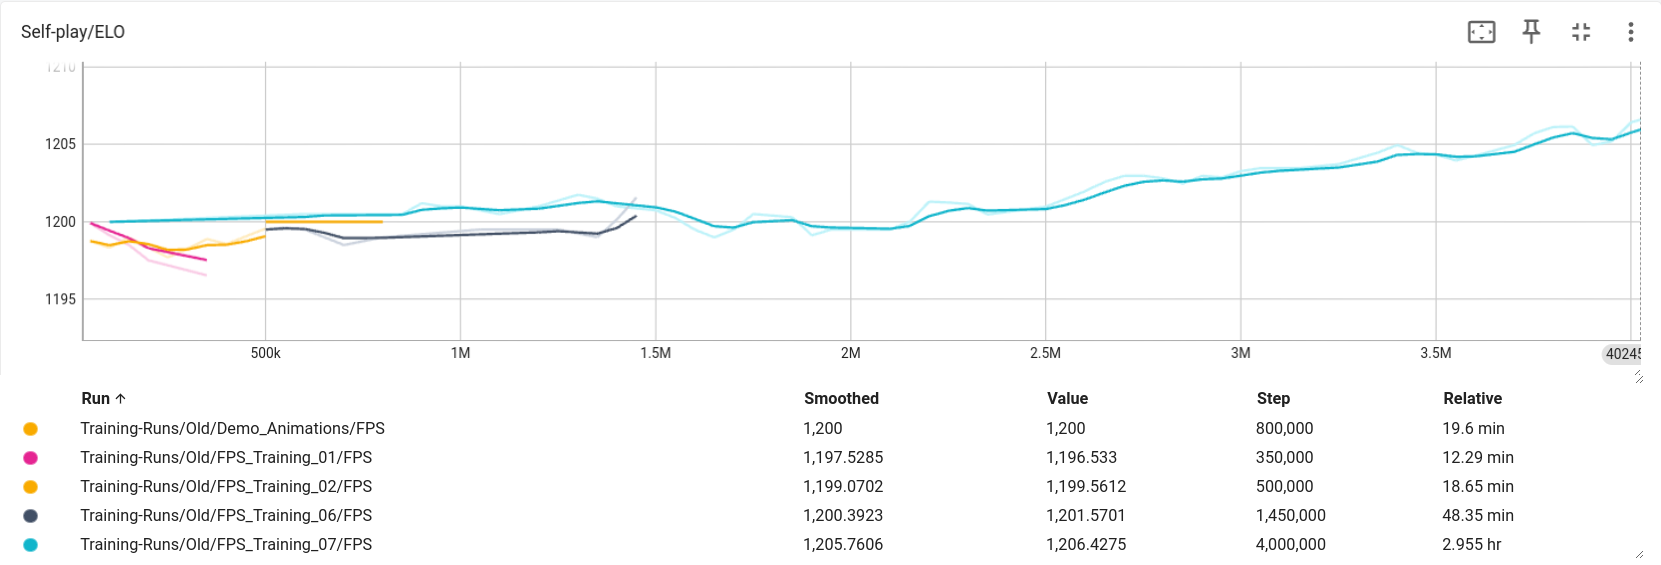
\includegraphics[width=0.5\linewidth]{phase2_results.png}
    \caption{\textit{Results for Phase 2}}
    \label{phase2}
\end{figure}
 
\begin{figure}
    \centering
    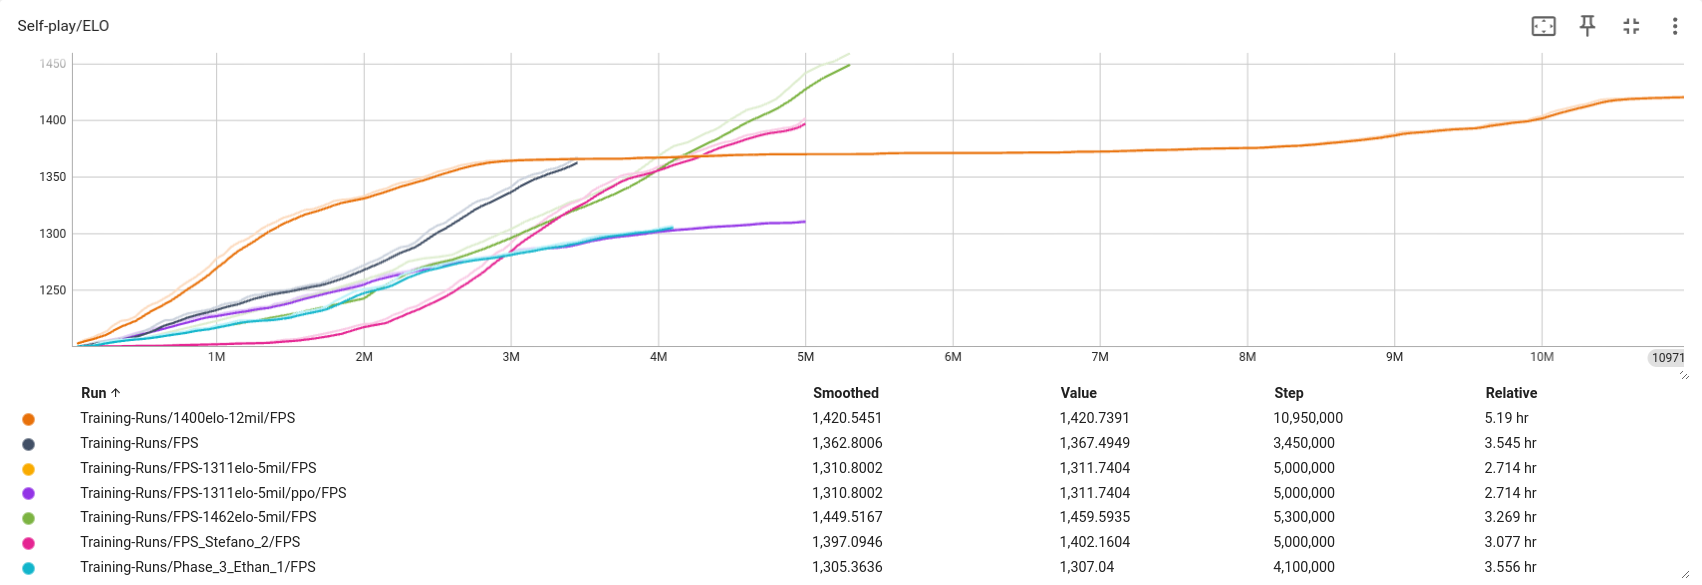
\includegraphics[width=0.5\linewidth]{phase3_results.png}
    \caption{\textit{Results for Phase 3}}
    \label{phase3}
\end{figure}



Cumulative reward is the sum of all points an agent receives from the reward structure in a given number of training iterations. Its formula is $$\sum\limits_{i\in I}k_{i}w_{i},$$ where $I$ is the set of all rewards and punishments, $k$ is the number of times each reward/punishment is given to the agent, and $w$ is the amount of points a certain reward/punishment is worth.

% 6. Discussion
\section{Discussion}
\begin{itemize}
    \item Interpret results:
    \item Answer research questions.
    \item Explain findings with evidence.
    \item Advancing the field:
    \item Highlight novelty factors.
    \item Address discrepancies with prior work.
    \item Issues and limitations:
    \item Report unexpected results and solutions.
    \item Identify study limitations and propose future directions.
\end{itemize}

% 7. Conclusion
\section{Conclusion}
\begin{itemize}
    \item Summary: Recap main results (answer "What?").
    \item Conclusion: Discuss implications (answer "So what?").
    \item Outlook: Suggest future research and improvements.
    \item Note: Avoid introducing new information.
\end{itemize}
Our project shows that agents can be trained using adversarial techniques and reinforcement learning on the Unity game engine. To extend the engine with the necessary tools, we used Unity's ML-Agents library. For our first research question, we showed that Unity's ML-Agents library offers sufficient infrastructure to train an agent for any given task. The library does this by allowing us to write customer sensors for the agent that record input data, using this data with machine learning algorithms to train the agent, and then having the agent perform some specified action.  

We also ran experiments to test the feasibility of machine learning solutions as a substitute for traditional decision tree-based AI in videos games. Our results indicate that while generative AI plays well from a technical perspective, but is still unable to capture the fluidity of action that makes NPCs immersive and realistic, thus making it look jilted and stiff from a player's perspective. As things currently stand, our experiment was not able to prove that generative AI is a good substitute for normal AI, but we also faced significant technical limitations during coding that limited our ability to train our agents. It is possible that given more time and computing resources, we could train a generative AI model that parallels normal AI from both a technical and player perspective.

% 8. Appendix
\section{Appendix}
\begin{itemize}
    \item Additional material:
    \item Raw data.
    \item (Pseudo)-code.
    \item Extra tables/figures.
    \item Labeling: Refer to appendices in the main text.
\end{itemize}

% 9. References
\newpage
\addcontentsline{toc}{section}{References}
\bibliographystyle{plain}
\bibliography{references}  
\end{document}
